%%
%% This is file `tikzposter-template.tex',
%% generated with the docstrip utility.
%%
%% The original source files were:
%%
%% tikzposter.dtx  (with options: `tikzposter-template.tex')
%%
%% This is a generated file.
%%
%% Copyright (C) 2014 by Pascal Richter, Elena Botoeva, Richard Barnard, and Dirk Surmann
%%
%% This file may be distributed and/or modified under the
%% conditions of the LaTeX Project Public License, either
%% version 2.0 of this license or (at your option) any later
%% version. The latest version of this license is in:
%%
%% http://www.latex-project.org/lppl.txt
%%
%% and version 2.0 or later is part of all distributions of
%% LaTeX version 2013/12/01 or later.
%%


\documentclass{tikzposter} %Options for format can be included here

\usepackage{todonotes}

\usepackage[tikz]{bclogo}
\usepackage{lipsum}
\usepackage{amsmath}

\usepackage{booktabs}
\usepackage{longtable}
\usepackage[absolute]{textpos}
\usepackage[it]{subfigure}
\usepackage{graphicx}
\usepackage{cmbright}
%\usepackage[default]{cantarell}
%\usepackage{avant}
%\usepackage[math]{iwona}
\usepackage[math]{kurier}
\usepackage[T1]{fontenc}


%% add your packages here
\usepackage{hyperref}
% for random text
\usepackage{lipsum}
\usepackage[english]{babel}
\usepackage[pangram]{blindtext}

\colorlet{backgroundcolor}{blue!10}

 % Title, Author, Institute
\title{Air Pollution Measurements Prediction}
\author{Yu Li$^1$}
\institute{$^1$ Nanjing University of Science and Technology, China
}
%\titlegraphic{logos/tulip-logo.eps}

%Choose Layout
\usetheme{Wave}

%\definebackgroundstyle{samplebackgroundstyle}{
%\draw[inner sep=0pt, line width=0pt, color=red, fill=backgroundcolor!30!black]
%(bottomleft) rectangle (topright);
%}
%
%\colorlet{backgroundcolor}{blue!10}

\begin{document}


\colorlet{blocktitlebgcolor}{blue!23}

 % Title block with title, author, logo, etc.
\maketitle

\begin{columns}
 % FIRST column
\column{0.5}% Width set relative to text width

%%%%%%%%%% -------------------------------------------------------------------- %%%%%%%%%%
 %\block{Main Objectives}{
%  	      	\begin{enumerate}
%  	      	\item Formalise research problem by extending \emph{outlying aspects mining}
%  	      	\item Proposed \emph{GOAM} algorithm is to solve research problem
%  	      	\item Utilise pruning strategies to reduce time complexity
%  	      	\end{enumerate}
%%  	      \end{minipage}
%}
%%%%%%%%%% -------------------------------------------------------------------- %%%%%%%%%%


%%%%%%%%%% -------------------------------------------------------------------- %%%%%%%%%%
\block{Introduction}{
    In this competition you are predicting the values of air pollution measurements over time, 
    based on basic weather information (temperature and humidity) and the input values of 5 sensors.
    The three target values to you to predict are:
  	
  	\begin{description}
  	\item[target-carbon-monoxide] 
  	\item[target-benzene]
  	\item[target-nitrogen-oxides] 
  	\end{description}


}
%%%%%%%%%% -------------------------------------------------------------------- %%%%%%%%%%


%%%%%%%%%% -------------------------------------------------------------------- %%%%%%%%%%
\block{Data Description}{
\begin{minipage}{0.5\linewidth}
	Train:
\begin{tabular}{c| c }
	\toprule
	%\centering
	Elements & \texttt{Number}  \\
	\midrule
	$date time$
	&  {$7111$} \\
	$deg C$
	&  {$408$} \\
	$relative humidity$
	&  {$762$}  \\
	$absolute humidity$
	&  {$5451$}  \\
	$sensor 1$
	&  {$3882$} \\
	$sensor 2$
	&  {$3882$} \\
	$sensor 3$
	&  {$3882$} \\
	$sensor 4$
	&  {$3882$} \\
	$sensor 5$
	&  {$3882$} \\
	$target carbon monoxide$
	&  {$95$} \\
	$target benzene$
	&  {$405$} \\
	$target nitrogen oxides$
	&  {$3268$} \\
	\bottomrule
\end{tabular}
\end{minipage}
\begin{minipage}{0.5\linewidth}
	Test:
	\begin{tabular}{c| c }
		\toprule
		%\centering
		Elements & \texttt{Number}  \\
		\midrule
		$date time$
		&  {$2247$} \\
		$deg C$
		&  {$280$} \\
		$relative humidity$
		&  {$653$}  \\
		$absolute humidity$
		&  {$1915$}  \\
		$sensor 1$
		&  {$1758$} \\
		$sensor 2$
		&  {$1816$} \\
		$sensor 3$
		&  {$1833$} \\
		$sensor 4$
		&  {$1877$} \\
		$sensor 5$
		&  {$2017$} \\
		\bottomrule
	\end{tabular}
\end{minipage}
}
%%%%%%%%%% -------------------------------------------------------------------- %%%%%%%%%%


%%%%%%%%%% -------------------------------------------------------------------- %%%%%%%%%%

%\note{Note with default behavior}

%\note[targetoffsetx=12cm, targetoffsety=-1cm, angle=20, rotate=25]
%{Note \\ offset and rotated}

 % First column - second block


%%%%%%%%%% -------------------------------------------------------------------- %%%%%%%%%%
\block{Data Visualization}{

\begin{tikzfigure}
  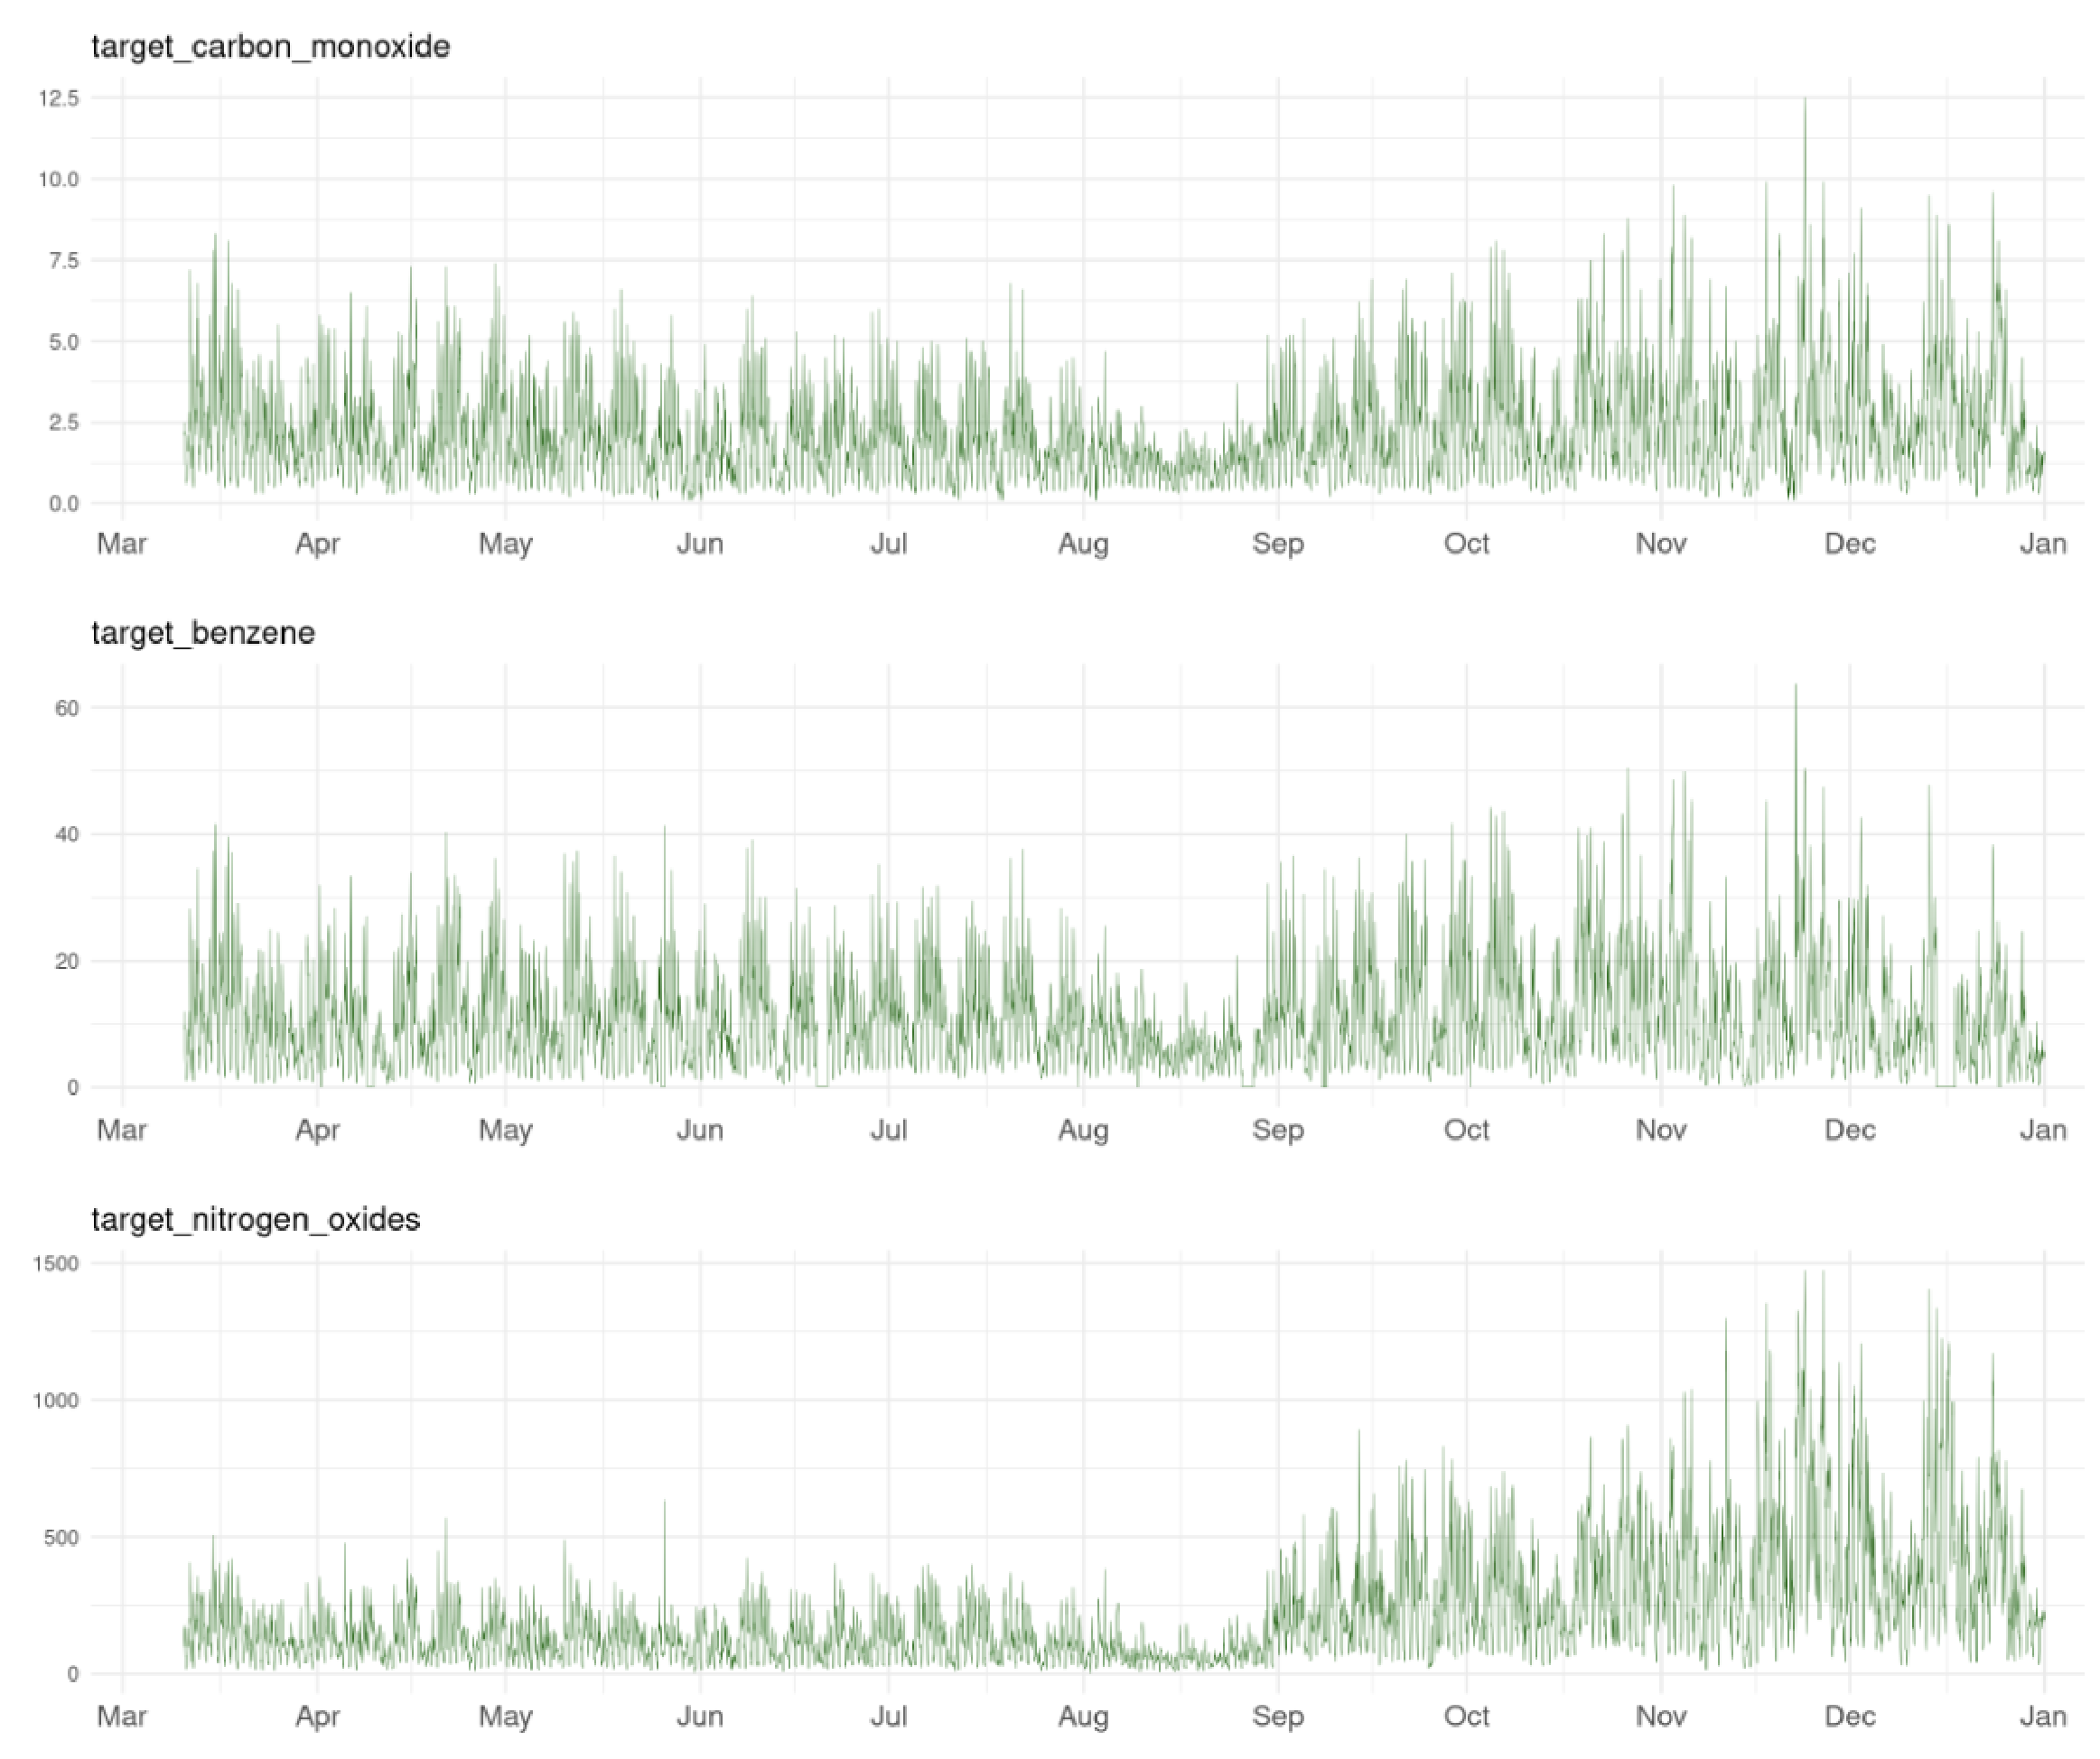
\includegraphics[scale=1.0]{figures//p1.eps}
\end{tikzfigure}


		
\begin{description}
  	\item[Overall Situation]
  	It can be seen from the figure that the values of the three target pollutants in August each year will be lower, 
  	gradually rising from September, and significantly higher than the level before August, 
  	so it is necessary to take the month as a feature of the model. 
\end{description}

}
%%%%%%%%%% -------------------------------------------------------------------- %%%%%%%%%%


% SECOND column
\column{0.5}
 %Second column with first block's top edge aligned with with previous column's top.

%%%%%%%%%% -------------------------------------------------------------------- %%%%%%%%%%
\block{Data Visualization}{

\begin{tikzfigure}
	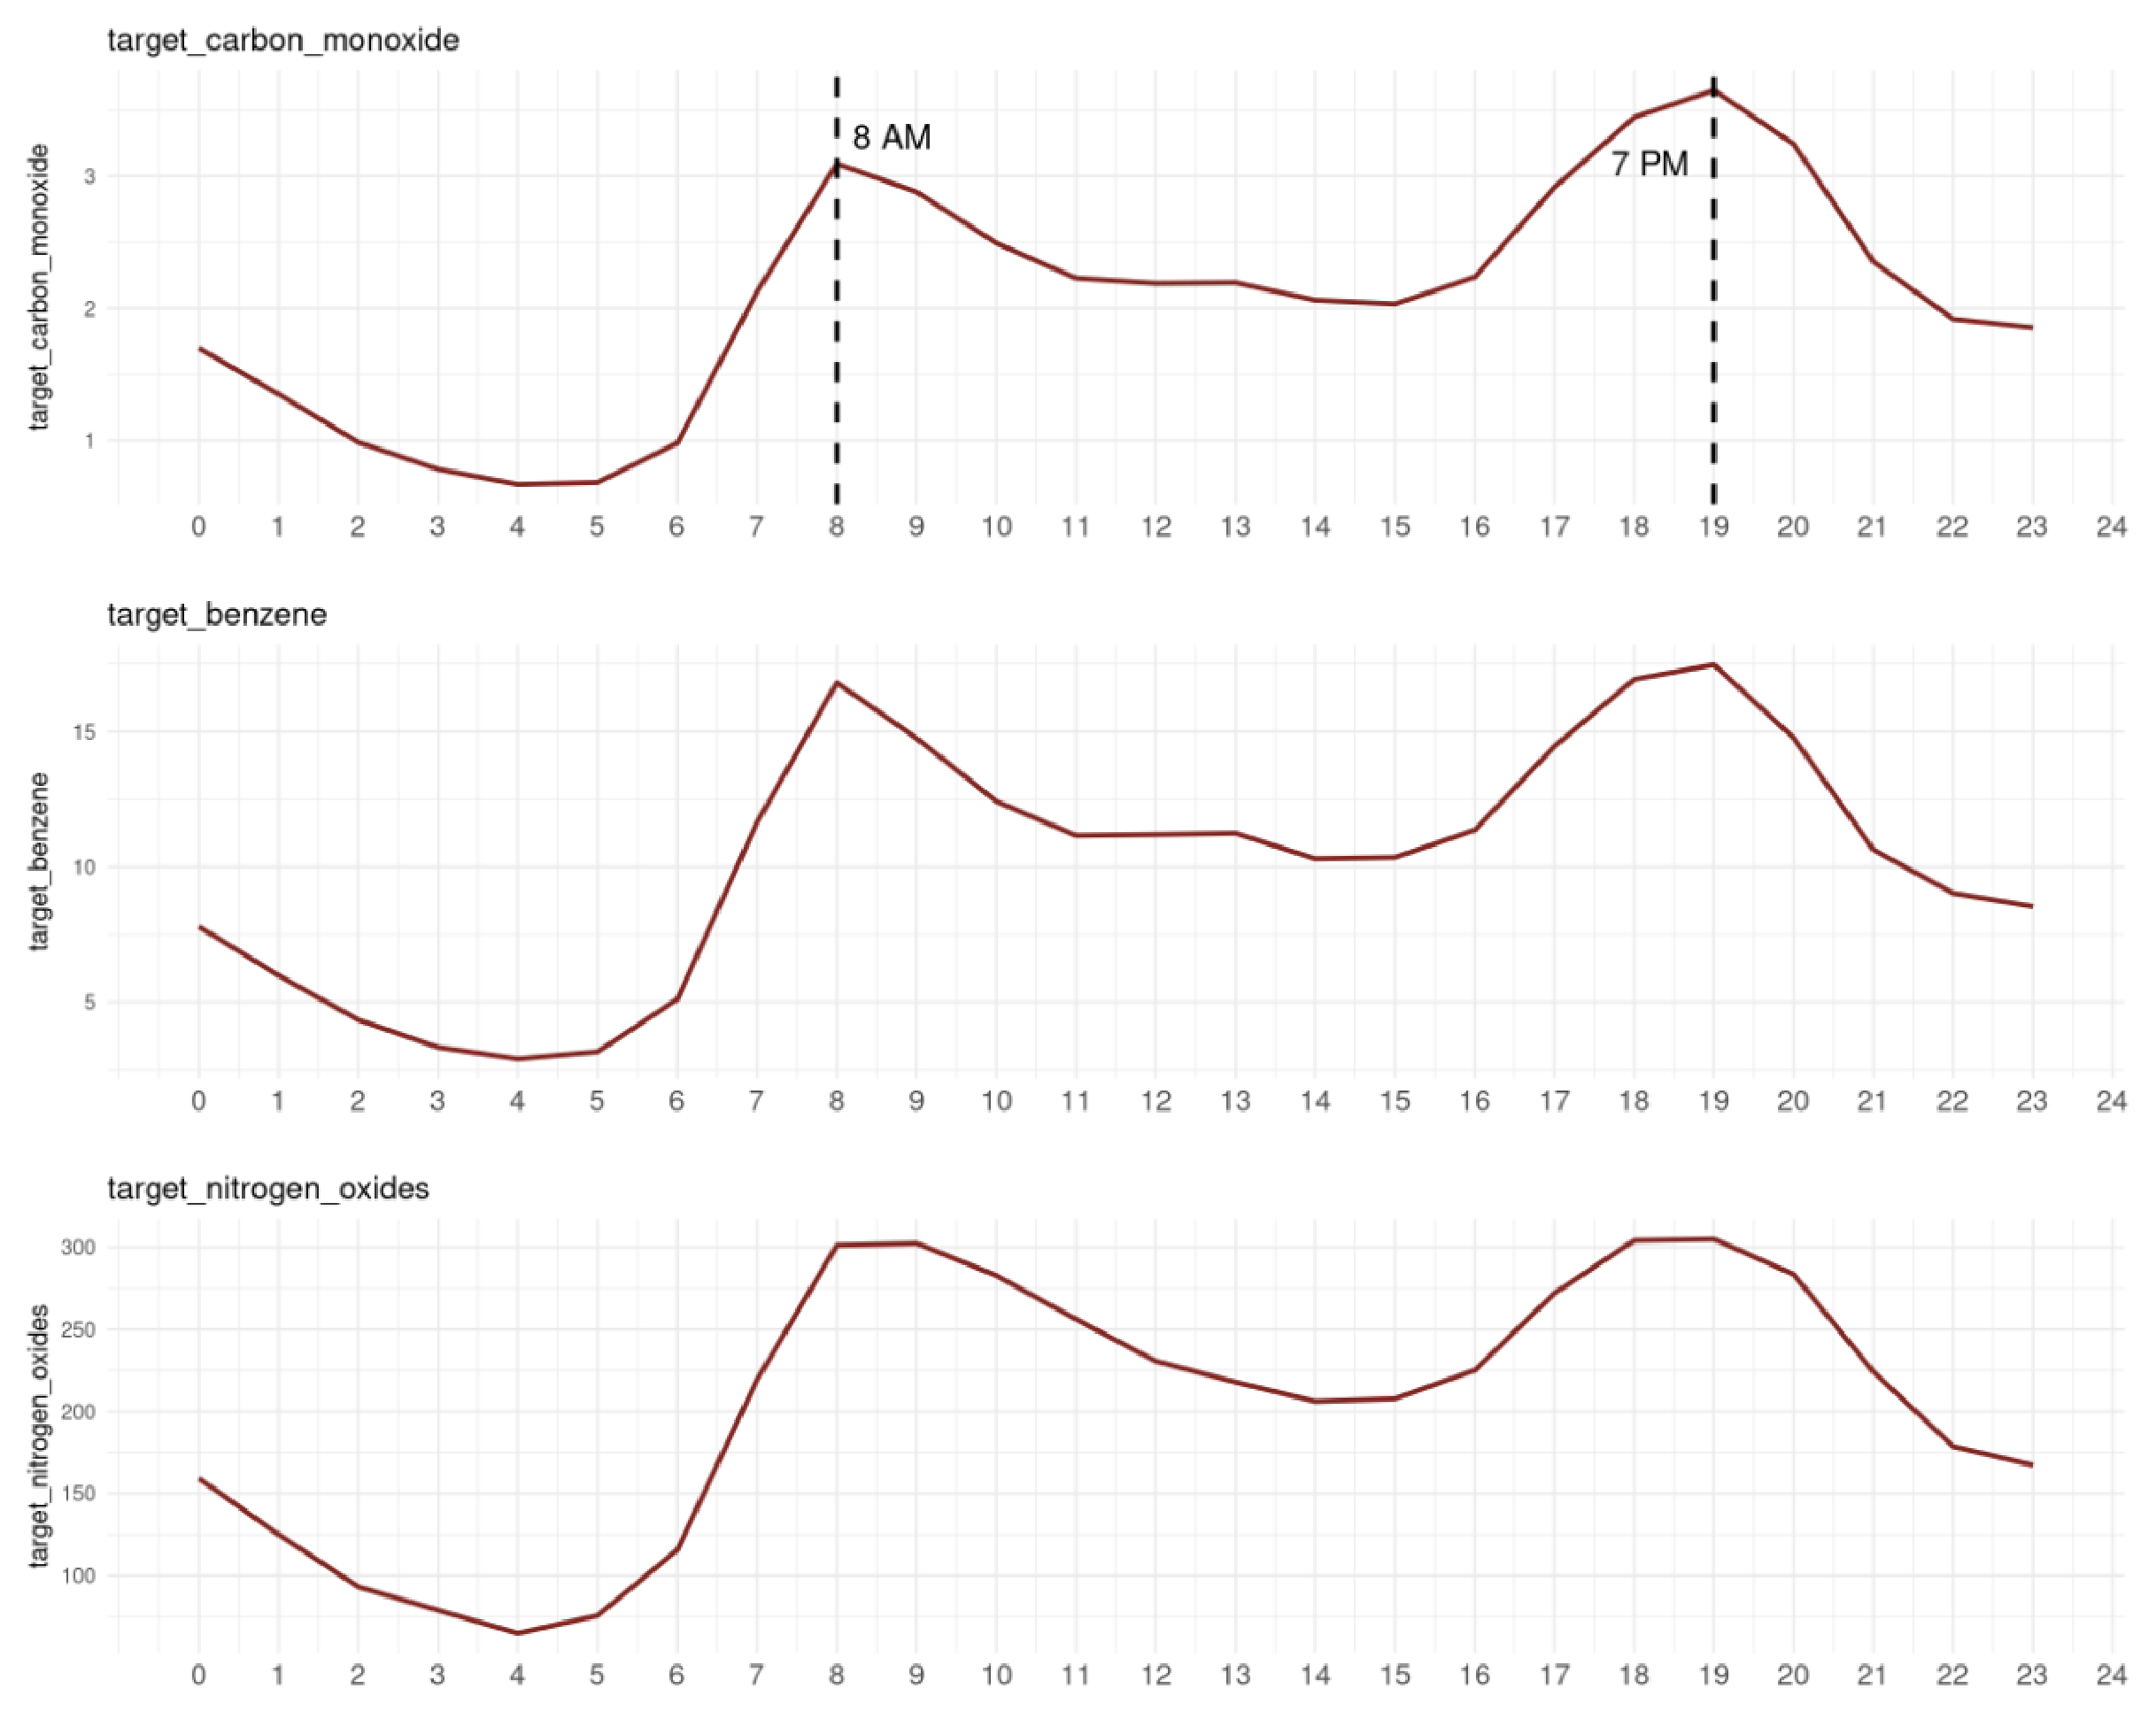
\includegraphics[scale=1.0]{figures//p5.eps}
\end{tikzfigure}

\begin{description}
	\item[Daily Situation]
	It can be seen from the figure that the level of each pollutant is the lowest at 5:00 a.m. every day, and then gradually rises to 8:00 a.m. to reach the first peak, and then gradually falls to 4:00 p.m., and then rises to 7:00 p.m. to reach the second peak, and then continues to decline, so it is necessary to take time as a feature of the model.
\end{description}

}
%%%%%%%%%% -------------------------------------------------------------------- %%%%%%%%%%
% Second column - first block


%%%%%%%%%% -------------------------------------------------------------------- %%%%%%%%%%
\block[titleleft]{Feature and Model}
{
\begin{description}
	\item[Features] 
	According to the analysis of training data, the following features are used for model training:
	 absolute-humidity, 
	 deg-C, 
	 relative-humidity, 
	 sensor1-5, 
	 month, 
	 week, 
	 is-weekend, 
	 hour
\end{description}

\vspace{.5cm}
\begin{description}
  	\item[LGBMRegressor] 
  	Data fitting using LGBMRegressor, the algorithm is easy to use. 
  	It only needs to put the set features and three prediction targets into the model for training, 
  	but there is no parameter optimization, which has a certain impact on the training results.
\end{description}


}
%%%%%%%%%% -------------------------------------------------------------------- %%%%%%%%%%


% Second column - second block
%%%%%%%%%% -------------------------------------------------------------------- %%%%%%%%%%
\block[titlewidthscale=1, bodywidthscale=1]
{Result}
{
\begin{description}
  \item[Evaluation]
  Use RMSLE(Root Mean Squared Logarithmic Error) to evaluate the results
  \begin{tikzfigure}
  	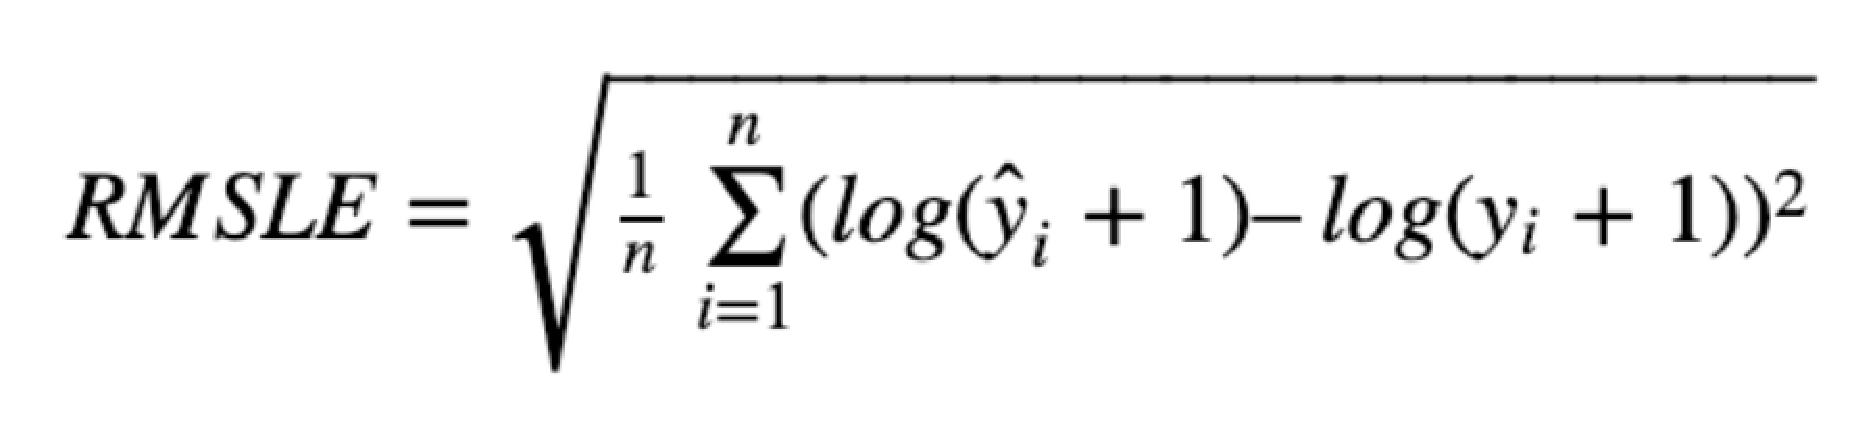
\includegraphics[scale=1.0]{figures//RMSLE.eps}
  \end{tikzfigure}

  \item[Private Score]
  :0.33979

  \item[Public Score]
  :0.387
\end{description}
}
%%%%%%%%%% -------------------------------------------------------------------- %%%%%%%%%%


% Bottomblock
%%%%%%%%%% -------------------------------------------------------------------- %%%%%%%%%%


%\note[targetoffsetx=8cm, targetoffsety=-10cm,rotate=0,angle=180,radius=8cm,width=.46\textwidth,innersep=.1cm]{
%Acknowledgement
%}

%\block[titlewidthscale=0.9, bodywidthscale=0.9]
%{Acknowledgement}{
%}
%%%%%%%%%% -------------------------------------------------------------------- %%%%%%%%%%

\end{columns}


%%%%%%%%%% -------------------------------------------------------------------- %%%%%%%%%%
%[titleleft, titleoffsetx=2em, titleoffsety=1em, bodyoffsetx=2em,%
%roundedcorners=10, linewidth=0mm, titlewidthscale=0.7,%
%bodywidthscale=0.9, titlecenter]

%\colorlet{noteframecolor}{blue!20}
\colorlet{notebgcolor}{blue!20}
\colorlet{notefrcolor}{blue!20}
\note[targetoffsetx=-13cm, targetoffsety=-13cm,rotate=0,angle=180,radius=8cm,width=.96\textwidth,innersep=.4cm]
{
\begin{minipage}{0.3\linewidth}
\centering

\includegraphics[width=24cm]{./graphics/logos/tulip-wordmark.eps}
\end{minipage}
\begin{minipage}{0.7\linewidth}
{ \centering
 The $11^{th}$ International Conference on Knowledge Science,
  Engineering and Management (KSEM 2018),
  17-19/08/2018, Changchun, China
}
\end{minipage}
}
%%%%%%%%%% -------------------------------------------------------------------- %%%%%%%%%%


\end{document}

%\endinput
%%
%% End of file `tikzposter-template.tex'.
